\section{Introduction}

Over the past few decades, there has been a significant shift in computing and storage, transitioning from PC-like clients to smaller, often mobile devices, coupled with expansive internet services. 
Concurrently, traditional enterprises are increasingly embracing cloud computing.

This shift offers several user experience improvements, including ease of management and ubiquitous access.

For vendors, Software-as-a-Service (SaaS) facilitates faster application development, making changes and improvements easier. 
Moreover, software fixes and enhancements are streamlined within data centers, rather than needing updates across millions of clients with diverse hardware and software configurations. 
Hardware deployment is simplified to a few well-tested configurations.

Server-side computing enables the swift introduction of new hardware devices, such as hardware accelerators or platforms, and supports many application services running at a low cost per user.
Certain workloads demand substantial computing capability, making data centers a more natural fit compared to client-side computing.

\subsection{Warehouse-scale computers}
The rise of server-side computing and the widespread adoption of internet services have given rise to a new class of computing systems known as warehouse-scale computers (WSCs).
In warehouse-scale computing, the program:
\begin{itemize}
    \item Operates as an internet service.
    \item Can comprise tens or more individual programs.
    \item These programs interact to deliver complex end-user services like email, search, maps, or machine learning.
\end{itemize}
Data centers are facilities where numerous servers and communication units are housed together due to their shared environmental needs, physical security requirements, and for the sake of streamlined maintenance.
Traditional data centers typically accommodate a considerable number of relatively small- or medium-sized applications. 
Each application operates on a dedicated hardware infrastructure, isolated and safe guarded against other systems within the same facility. 
These applications typically do not communicate with one another. 
Moreover, these data centers host hardware and software for multiple organizational units or even different companies.

In contrast, warehouse-scale computers are owned by a single organization, employ a relatively uniform hardware and system software platform, and share a unified systems' management layer.
\begin{figure}[H]
    \centering
    \begin{subfigure}{0.49\textwidth}
        \centering
        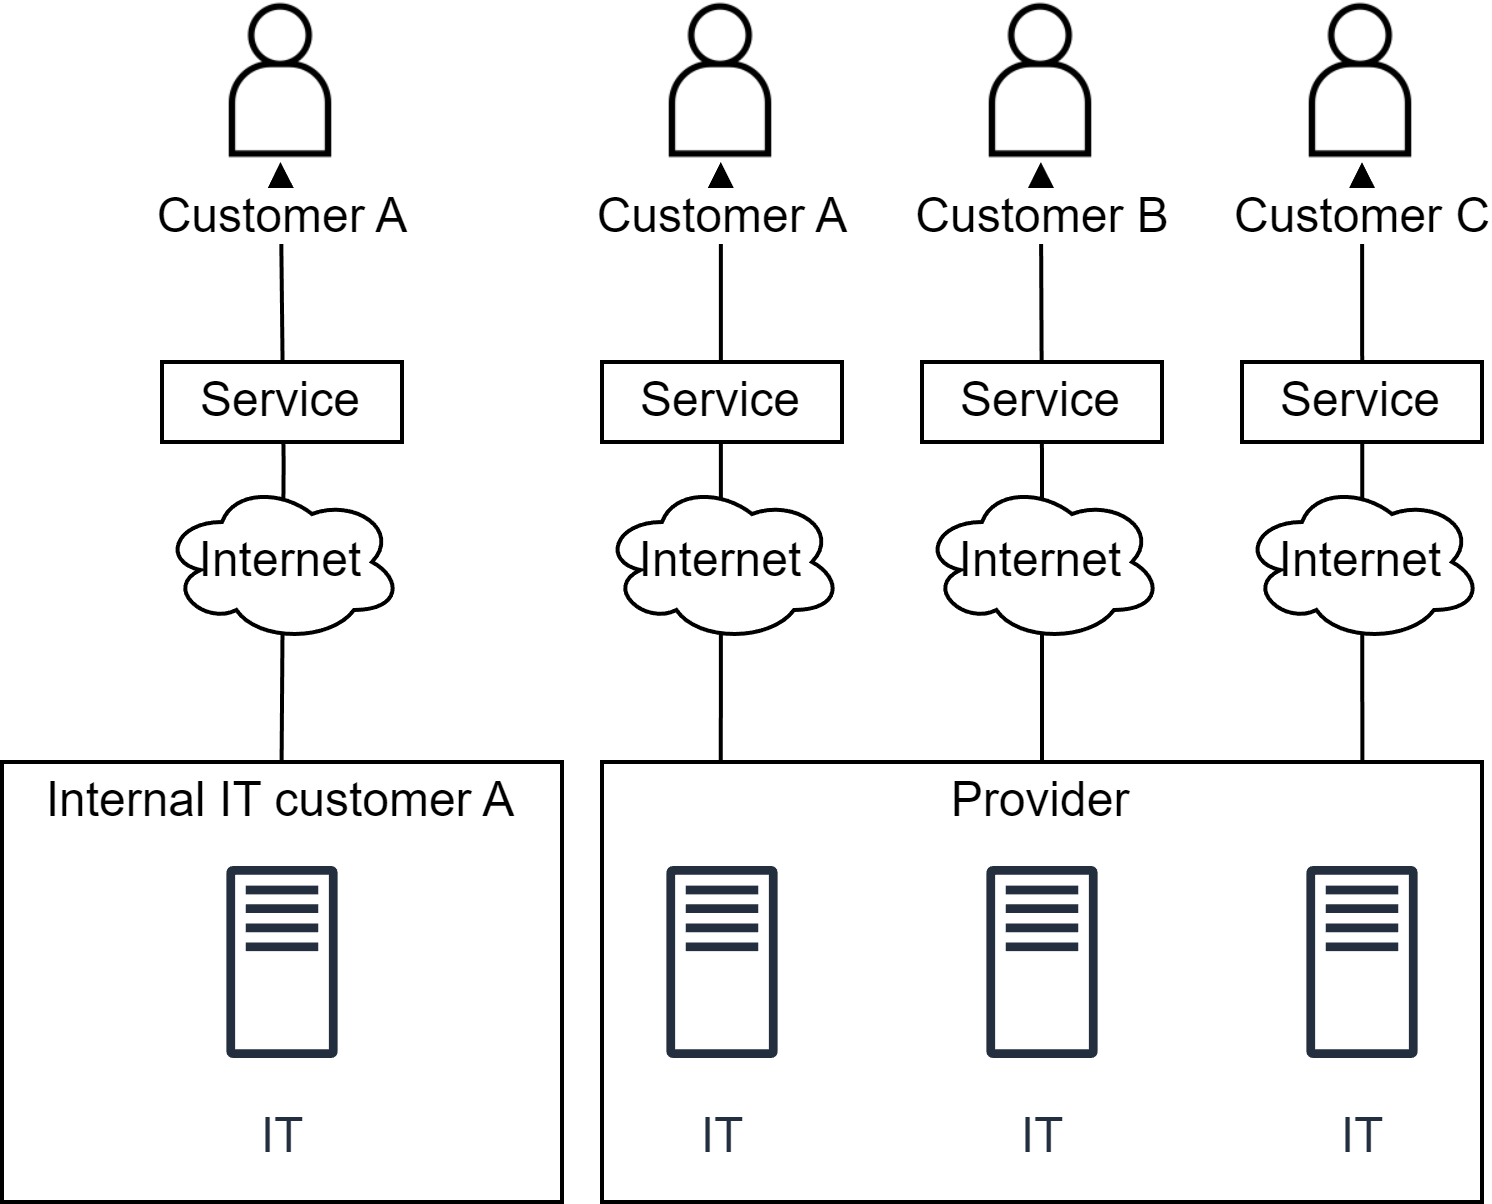
\includegraphics[width=0.75\linewidth]{images/datacenter.png} 
        \caption{Data center}
    \end{subfigure}
    \begin{subfigure}{0.49\textwidth}
        \centering
        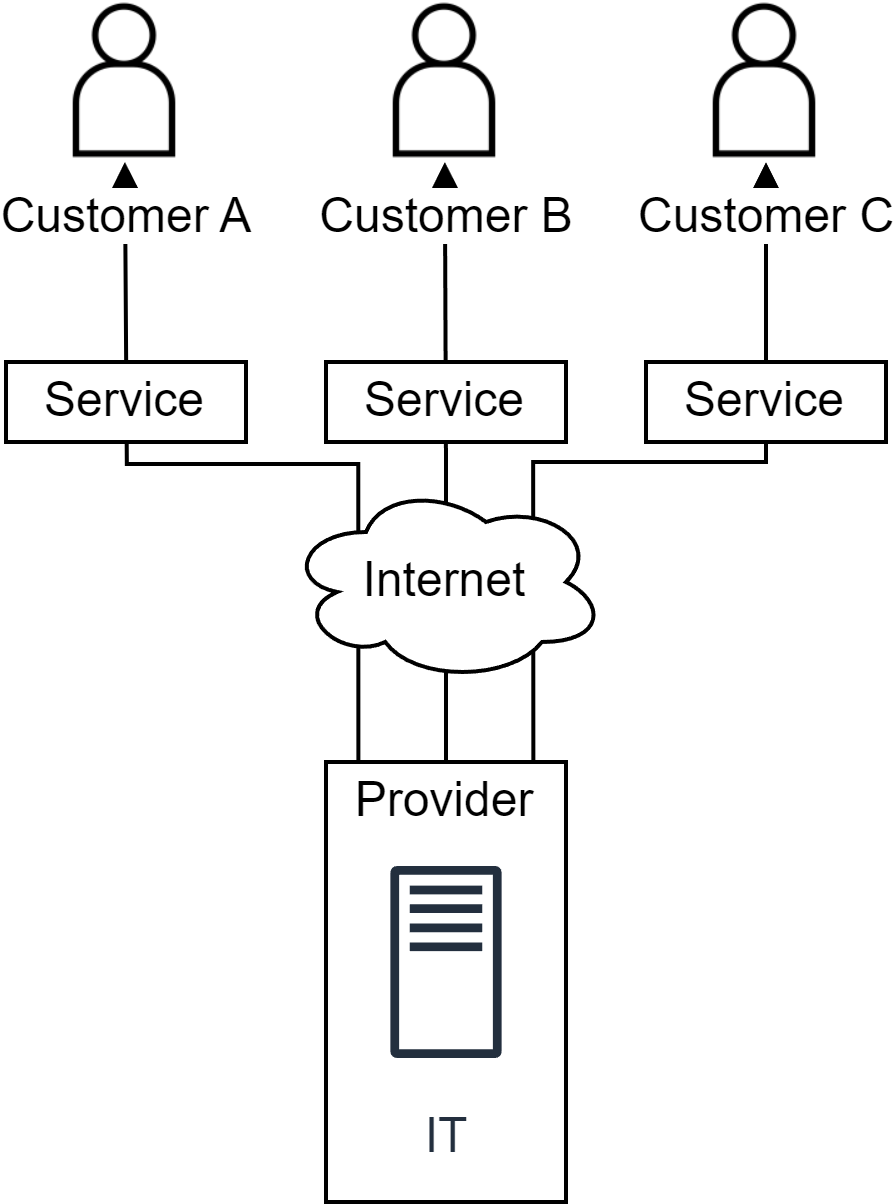
\includegraphics[width=0.45\linewidth]{images/warehouse.png}
        \caption{Data warehouse}
    \end{subfigure}
    \caption{Structures of data centers and data warehouses}
\end{figure}
Warehouse-scale computers operate a reduced quantity of highly expansive applications, often internet services.
Their shared resource management infrastructure affords considerable deployment flexibility. 
Designers are driven by the imperatives of homogeneity, single-organization control, and cost efficiency, prompting them to adopt innovative approaches in crafting WSCs.

Originally conceived for online data-intensive web workloads, warehouse-scale computers have expanded their capabilities to drive public cloud computing systems, such as those operated by Amazon, Google, and Microsoft. 
These public clouds do accommodate numerous small applications, resembling a traditional data center setup. 
However, all these applications leverage virtual machines or containers and access shared, large-scale services for functionalities like block or database storage and load balancing, aligning seamlessly with the WSC model.

The software operating on these systems is designed to run on clusters comprising hundreds to thousands of individual servers, far surpassing the scale of a single machine or a single rack. 
The machine itself constitutes this extensive cluster or aggregation of servers, necessitating its consideration as a single computing unit.

\subsection{Geographical distribution of data centers}
Frequently, multiple data centers serve as replicas of the same service, aiming to reduce user latency and enhance serving throughput. 
Requests are typically processed entirely within one data center.

\begin{definition}[\textit{Geographic area}]
    Geographic areas partition the world into sectors, each defined by geopolitical boundaries. 
\end{definition}

Within each geographic area, there are at least two computing regions.
Customers perceive regions as a more detailed breakdown of the infrastructure. 
Notably, multiple data centers within the same region are not externally visible. 
The perimeter of each computing region is defined by latency (with a round trip latency of two milliseconds), which is too far for synchronous replication but sufficient for disaster recovery.

\begin{definition}[\textit{Availability zone}]
    Availability zones represent more granular locations within a single computing region.
\end{definition}

They enable customers to operate mission-critical applications with high availability and fault tolerance to datacenter failures by providing fault-isolated locations with redundant power, cooling, and networking.
Application-level synchronous replication among availability zones is implemented, with a minimum of three zones being adequate for ensuring quorum.

\begin{figure}[H]
    \centering
    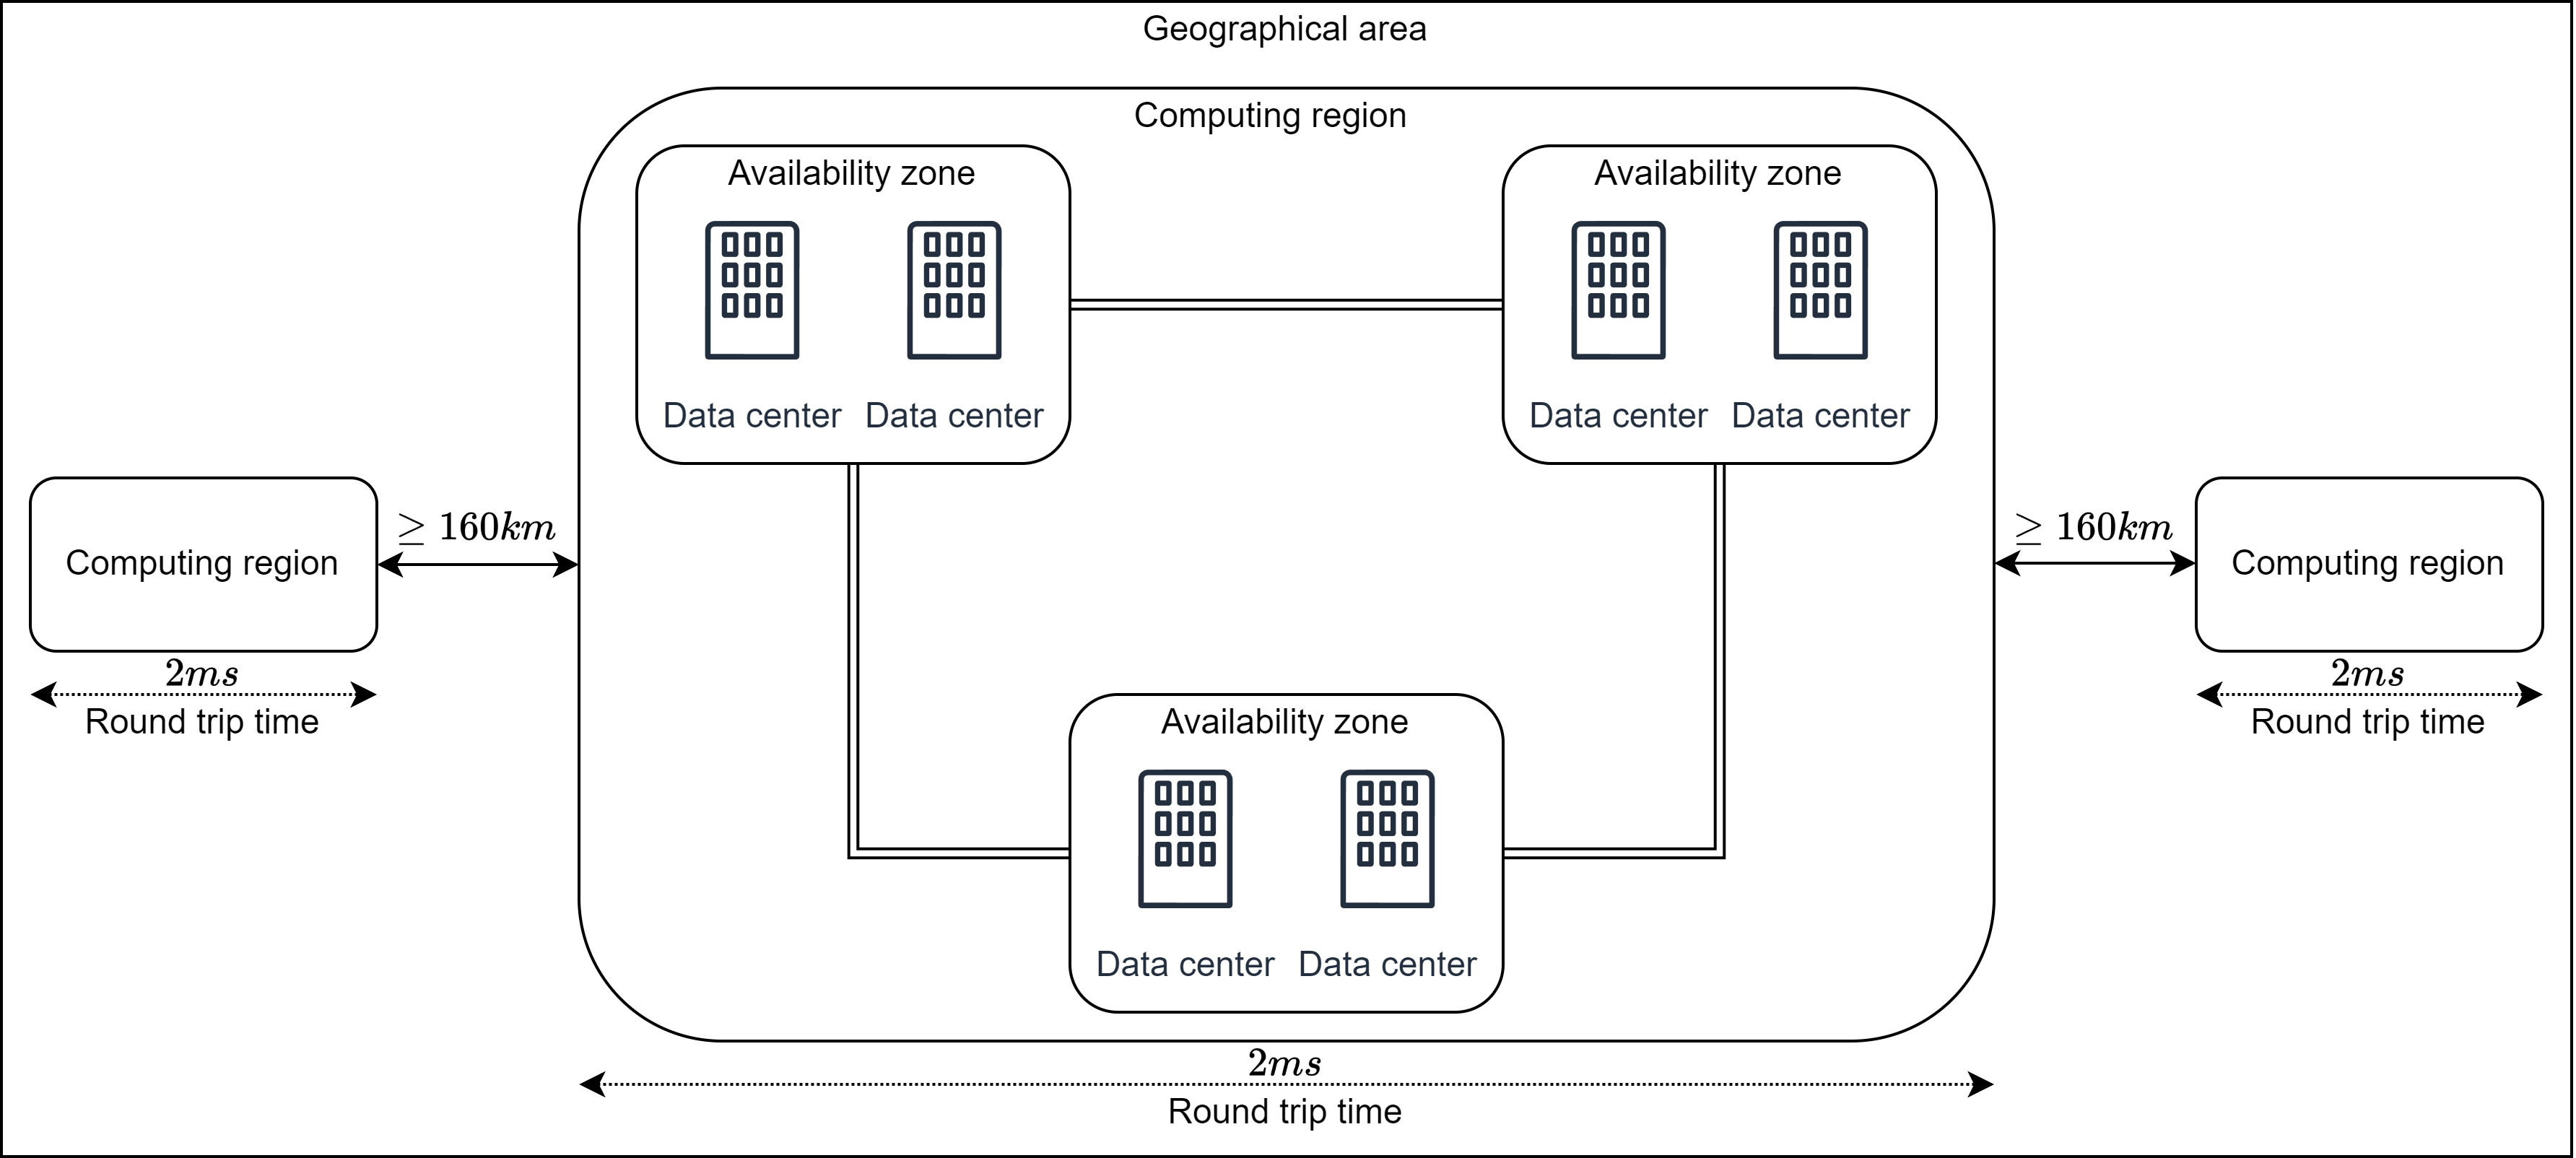
\includegraphics[width=1\linewidth]{images/computing.png}
    \caption{Geographical area structure}
\end{figure}